\begin{activity} \label{A:3.1.1}  Suppose that $g(x)$ is a function continuous for every value of $x \ne 2$ whose first derivative is $\ds g'(x) = \frac{(x+4)(x-1)^2}{x-2}$.  Further, assume that it is known that $g$ has a vertical asymptote at $x = 2$.
\ba
  \item Determine all critical values of $g$.
  \item By developing a carefully labeled first derivative sign chart, decide whether $g$ has  as a local maximum, local minimum, or neither at each critical value.
  \item Does $g$ have a global maximum? global minimum? Justify your claims.
  \item What is the value of $\ds \lim_{x \to \infty} g'(x)$?  What does the value of this limit tell you about the long-term behavior of $g$?
  \item Sketch a possible graph of $y = g(x)$.
\ea
\end{activity}
\begin{smallhint}
\ba
	\item For which $x$ is $g'(x) = 0$?
	\item Note that $(x-1)^2$ is positive for all $x \ne 1$.
	\item Use your first derivative sign chart from (b).
	\item Try expanding the numerator before evaluating the limit.
	\item Think carefully about the information from the sign chart found in (b).
\ea
\end{smallhint}
\begin{bighint}
\ba
	\item For which $x$ is $g'(x) = 0$?  Remember that a fraction's value is zero if and only if its numerator is zero.
	\item Note that $(x-1)^2$ is positive for all $x \ne 1$.  How do the signs of $(x+4)$ and $(x-2)$ then determine the overall sign of $g'(x)$?
	\item Use your first derivative sign chart from (b) and remember to the first derivative test.
	\item Try expanding the numerator before evaluating the limit and think about what you know about the limit of a rational function as $x \to \infty$.
	\item Focus on where $g$ is increasing and decreasing, along with where it must have a horizontal tangent line.
\ea
\end{bighint}
\begin{activitySolution}
\ba
  \item Since $\ds g'(x) = \frac{(x+4)(x-1)^2}{x-2}$, we see that $g'(x) = 0$ implies that $x = -4$ or $x = 1$.  While $x = 2$ makes $g'$ undefined, we are told that $g$ has a vertical asymptote at $x = 2$, so $x = 2$ is not in the domain of $g$, and hence is technically not a critical value of $g$.  Nonetheless, we place $x = 2$ on our first derivative sign chart since the vertical asymptote is a location at which $g'$ may change sign.
  \item The first derivative sign chart shows that $g'(x) > 0$ for $x < -4$, $g'(x) < 0$ for $-4 < x < 1$, $g'(x) < 0$ for $1 < x < 2$, and $g'(x) > 0$ for $x > 2$.  By the first derivative test, $g$ has a local maximum at $x = -4$ and neither a max nor min at $x = 1$.  As these are the only two critical values, these are the only two locations for possible extremes.  (Note: although $g$ changes from decreasing to increasing at $x = 2$, this is due to a vertical asymptote, and $g$ does not have a minimum there.)
  \item Because $g$ is decreasing as $x \to 2^-$ (where $g$ has a vertical asymptote), $g$ does not have a global minimum.  For $x > 2$, $g$ is always increasing, which suggests that $g$ does not have a global maximum (though we do not know for sure that $g$ increases without bound).
  \item We observe that
  \begin{eqnarray*} 
  	\lim_{x \to \infty} g'(x) & = & \lim_{x \to \infty} \frac{(x+4)(x-1)^2}{x-2} \\
					& = & \lim_{x \to \infty} \frac{x^3 + 2x^2 - 7x + 4}{x-2} \cdot \frac{\frac{1}{x}}{\frac{1}{x}} \\
					& = & \lim_{x \to \infty} \frac{x^2 + 2x - 7 + \frac{4}{x}}{1 - \frac{2}{x}} \\
					& = & \infty
  \end{eqnarray*}
Since $g'(x) \to \infty$ as $x \to \infty$, this tells us that $g$ increases without bound as $x \to \infty$.
  \item From all of our work above, we know that $g$ has a local maximum at $x = -4$, a horizontal tangent line with neither a max nor min at $x = 1$, and a vertical asymptote at $x = 2$, plus $g$ and $g'$ both increase without bound as $x \to \infty$.  Thus, a possible graph of $g$ is the following.
  \begin{center}
  	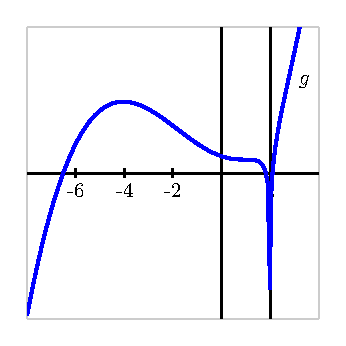
\includegraphics{figures/3_1_Act1Soln.eps}
  \end{center}
\ea
\end{activitySolution}
\aftera